\documentclass[aspectratio=169]{beamer}

%
% Choose how your presentation looks.
%
% For more themes, color themes and font themes, see:
% http://deic.uab.es/~iblanes/beamer_gallery/index_by_theme.html
%
\mode<presentation>
\mode<presentation>
{
  \usetheme[compress]{Ilmenau}      % or try Darmstadt, Madrid, Warsaw, ...
  \usecolortheme{beaver} % or try albatross, beaver, crane, ...
  \usefonttheme{default}  % or try serif, structurebold, ...
  \setbeamertemplate{navigation symbols}{}
  \setbeamertemplate{caption}[numbered]
} 
\usepackage[english]{babel}
\usepackage[utf8x]{inputenc}
\usepackage{graphicx}
\usepackage{setspace}
\usepackage{tikz} \usetikzlibrary{snakes}
\usepackage{epstopdf}
\usepackage[round]{natbib}
\setbeamertemplate{enumerate items}[circle]
\setbeamertemplate{itemize items}[circle]
\setbeamertemplate{blocks}[rounded][shadow=false] 
\usepackage{remreset}% tiny package containing just the \@removefromreset command
\makeatletter
\@removefromreset{subsection}{section}
\makeatother
\setcounter{subsection}{1}
\setbeamertemplate{section in toc}[sections numbered]


\usepackage[english]{babel}
\usepackage[utf8x]{inputenc}
\title[Housing bubbles]{Housing Bubbles and \\Support for Incumbents}
\author{\textbf{Frederik G. Hjorth} \and \textbf{Martin V. Larsen}}
\institute[UCPH]{\small Department of Political Science \\ University of Copenhagen}
\date[October 2015]{ 47th annual meeting of the DPSA \\ October 30th 2015}


\begin{document}
	
	\begin{frame}
		\titlepage
	\end{frame}
	
	
	\AtBeginSection[]{\begin{frame}{Outline}
			\tableofcontents[currentsection] 
		\end{frame}}
	
\section{Politicized homes?}

	\begin{frame}
	%{Politicized homes}
	Key economic feature of post-industrial societies: mass home ownership.
	
	\vspace{0.2in} 

	\begin{itemize}
		\item main form of capital ordinary people have.
		\item key part of one's control over one's immediate context.
		\item often the focus of political rhetoric.
	\end{itemize}
	
		\vspace{0.2in} \pause
		
	$\rightsquigarrow$ but: relatively little research on how home ownership shapes political behavior.
		\end{frame}	
	
		\begin{frame}
		\citet{ansell2014political}: house price appreciation reduces preferences for social insurance. 
		
		$\rightsquigarrow$ see also \citet{di2007formation}.
						
		\vspace{0.3in}	\pause
						
		Here: \emph{local house prices} and \emph{incumbent government support}.					
		
		\vspace{0.3in} \pause	
		
		Feeds into litrature on effect of local economic conditions \textit{vis-à-vis} personal or national.
       			
		\end{frame}	
		
		
	\begin{frame}

Usually, this literature on the effects of local economy uses...

		\vspace{0.3in}	\pause
		
		\begin{enumerate}[<+->]
			\item large contextual units: does not necessarily map on to voters' local community.
			\item within-unit variation: potentially confounding for several reasons.
			\item sample-based measures of local economy (although see \citealt{healy2014presidential})
		\end{enumerate}

		\vspace{0.3in}	\pause

 \pause These data constraints potentially make for unreliable effect estimates. \pause

$\rightsquigarrow$ which is in fact what we usually see.
			
	\end{frame}	
	
	\begin{frame}
			
	The data and methods used in this paper try to break these usual data constraints.
	
\vspace{0.3in}	\pause

We do so by focusing on the Danish case, for which we have zip-code lvl population based measures of house prices over time.
			
\vspace{0.3in}	\pause
			
	Caveat: We cant discern the exact mechanism is. Could be ego-, socio- or geotropic.
	$\rightsquigarrow$ We focus on establishing an effect.
	
	\end{frame}	
	
\section{About the Danish Case}	
\begin{frame}
In international comparison, DK's housing bubble exceptionally volatile:

\begin{center}
\includegraphics<1>[width=0.8\textwidth]{../../figures/intcomparison.png}
\end{center}
\end{frame}	
	
	\begin{frame}
However, still great variation within DK (across municipalities below).

	\begin{center}
\includegraphics<1-2>[width=0.9\textwidth]{../../figures/manylines_oneplot.eps}	
		\end{center}
		
		\pause Our focus is on parliamentary elections in 2005, '07, '11 and '15.
	\end{frame}	
	
	
	
\section{Data}	
\begin{frame}
DV is electoral support for governing parties at individual precincts across the four Parliamentary elections.

\vspace{0.2in} \pause
Data is from Political-Ecological Data Archive (PEDA)  \pause

$\rightsquigarrow$ using this database we can create a balanced panel of precincts across elections.

\vspace{0.2in} \pause

PEDA also gives info on: avg. income, avg. wealth, pct. working and pct. on benefits. \pause

$\rightsquigarrow$ at the district level, only measured in 2011!

\end{frame}	

\begin{frame}
IV is year-over-year changes in the price of real-estate sold in the precinct's zip code.

\vspace{0.2in} \pause
Data is from the Danish Mortgage federation (Realkreditfordeling).  \pause

$\rightsquigarrow$ i.e. we have weighted avg. price of each quarter of condos and houses sold in zip. \pause

$\rightsquigarrow$ use price difference btwn prices in election-quarter and prices one year before. \pause

$\rightsquigarrow$ also measure price volatility; std. dev. of prices across the last eight quarters. 

\vspace{0.2in} \pause
We link precincts to zip-codes by identifying the zip code of the precinct's polling place.

\end{frame}	

\begin{frame}
\begin{center}
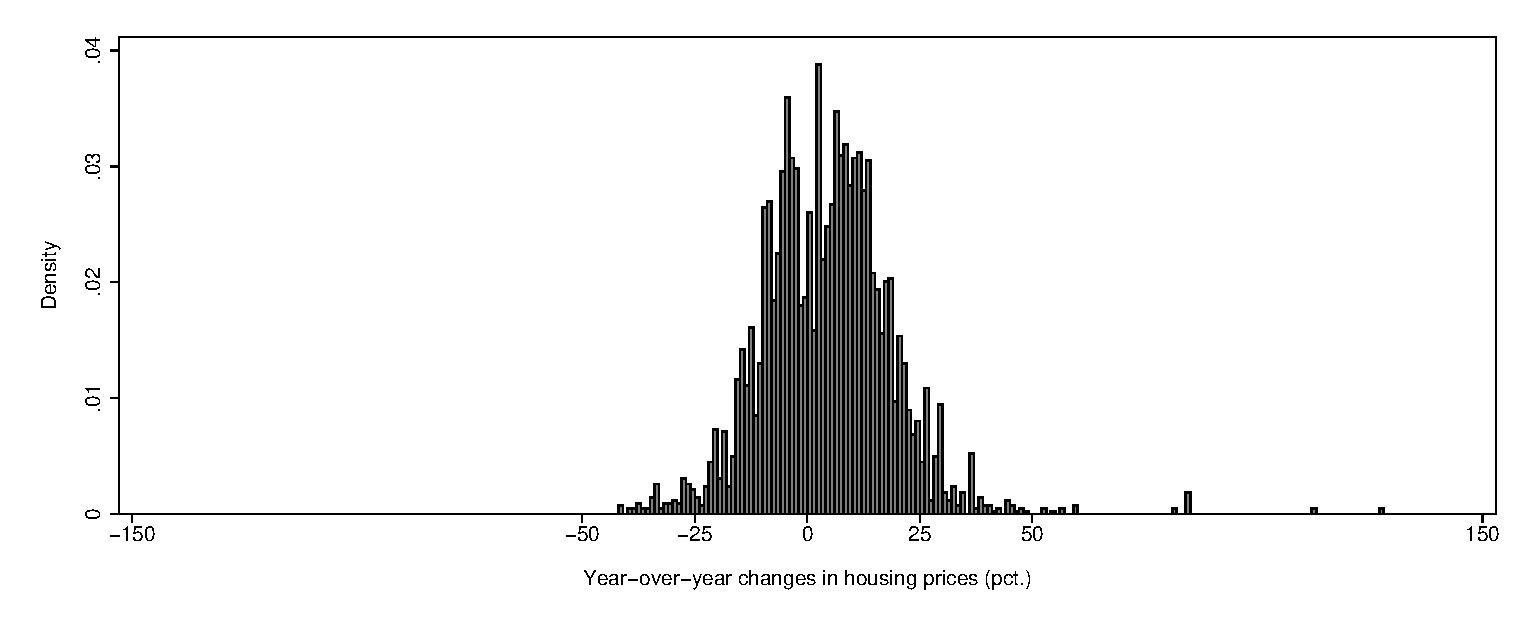
\includegraphics[width=0.9\textwidth]{../../figures/hphist.eps}	

$\mu=0.04$ \hspace{0.1in} $\sigma=0.14$
\end{center}
\end{frame}	


\section{Results}
\begin{frame}
	\footnotesize
		\only<1>{\begin{table}[htbp]\centering
\def\sym#1{\ifmmode^{#1}\else\(^{#1}\)\fi}
\caption{Estimated effects of house prices on electoral support for governing parties.} \label{tab1}
\begin{tabular}{l*{5}{c}}
\hline\hline
                    &\multicolumn{1}{c}{(1)}        &\multicolumn{1}{c}{(2)}        &\multicolumn{1}{c}{(3)}        &\multicolumn{1}{c}{(4)}        &\multicolumn{1}{c}{(5)}        \\
\hline
$\Delta$ house price&        0.10\sym{**}&        0.12\sym{**}&        0.05\sym{**}&        0.05\sym{**}&        0.01\sym{*} \\
                    &      (0.01)        &      (0.01)        &      (0.01)        &      (0.01)        &      (0.01)        \\
[1em]
\hline Precinct FE  &                    &$\checkmark$        &$\checkmark$        &$\checkmark$        &$\checkmark$        \\
[1em]
Year FE             &                    &                    &$\checkmark$        &$\checkmark$        &$\checkmark$        \\
[1em]
Year FE * Structural factors&                    &                    &                    &$\checkmark$        &$\checkmark$        \\
[1em]
Year FE * Municipality FE&                    &                    &                    &                    &$\checkmark$        \\
\hline
Observations        &        4192        &        4192        &        4192        &        4170        &        4170        \\
RMSE                &        8.40        &        7.16        &        5.71        &        4.77        &        2.84        \\
\hline\hline
\multicolumn{6}{l}{\footnotesize Standard errors in parentheses}\\
\multicolumn{6}{l}{\footnotesize \sym{*} \(p<0.05\), \sym{**} \(p<0.01\)}\\
\end{tabular}
\end{table}
}
		\only<2>{\begin{table}[htbp]\centering
\def\sym#1{\ifmmode^{#1}\else\(^{#1}\)\fi}
\caption{Estimated effects of house prices on electoral support for governing parties at t+1.} \label{tab2}
\begin{tabular}{l*{5}{c}}
\hline\hline
                    &\multicolumn{1}{c}{(1)}        &\multicolumn{1}{c}{(2)}        &\multicolumn{1}{c}{(3)}        &\multicolumn{1}{c}{(4)}        &\multicolumn{1}{c}{(5)}        \\
\hline
$\Delta$ house price&        0.12\sym{**}&        0.14\sym{**}&       -0.02        &       -0.01        &        0.02        \\
                    &      (0.01)        &      (0.01)        &      (0.01)        &      (0.01)        &      (0.01)        \\
[1em]
\hline Precinct FE  &                    &$\checkmark$        &$\checkmark$        &$\checkmark$        &$\checkmark$        \\
[1em]
Year FE             &                    &                    &$\checkmark$        &$\checkmark$        &$\checkmark$        \\
[1em]
Year FE * Structural factors&                    &                    &                    &$\checkmark$        &$\checkmark$        \\
[1em]
Year FE * Municiplaity FE&                    &                    &                    &                    &$\checkmark$        \\
\hline
Observations        &        3227        &        3227        &        3227        &        3209        &        3209        \\
RMSE                &        8.62        &        7.11        &        6.22        &        5.24        &        3.05        \\
\hline\hline
\multicolumn{6}{l}{\footnotesize Standard errors in parentheses}\\
\multicolumn{6}{l}{\footnotesize \sym{*} \(p<0.05\), \sym{**} \(p<0.01\)}\\
\end{tabular}
\end{table}
}
		\only<3>{\begin{table}[htbp]\centering
\def\sym#1{\ifmmode^{#1}\else\(^{#1}\)\fi}
\caption{Estimated effects of house prices on electoral support for governing parties at t-1.} \label{tab3}
\begin{tabular}{l*{4}{c}}
\hline\hline
                    &\multicolumn{1}{c}{(1)}        &\multicolumn{1}{c}{(2)}        &\multicolumn{1}{c}{(3)}        &\multicolumn{1}{c}{(4)}        \\
\hline
$\Delta$ house price&       -0.03\sym{**}&       -0.04\sym{**}&        0.07\sym{**}&        0.08\sym{**}\\
                    &      (0.01)        &      (0.01)        &      (0.01)        &      (0.01)        \\
[1em]
\hline Precinct FE  &                    &$\checkmark$        &$\checkmark$        &$\checkmark$        \\
[1em]
Year FE             &                    &                    &$\checkmark$        &$\checkmark$        \\
[1em]
Year FE * Structural factors&                    &                    &                    &$\checkmark$        \\
\hline
Observations        &        4197        &        4197        &        4197        &        4173        \\
RMSE                &        8.80        &        7.50        &        6.46        &        5.04        \\
\hline\hline
\multicolumn{5}{l}{\footnotesize Standard errors in parentheses}\\
\multicolumn{5}{l}{\footnotesize \sym{*} \(p<0.05\), \sym{**} \(p<0.01\)}\\
\end{tabular}
\end{table}
}
\end{frame}		

\begin{frame}
We examine two types of heterogeneity in this effect: negativity and volatility.

\vspace{0.3in} \pause

Negativity bias is prevalent in economic voting literature \citep[e.g.][]{bloom1975voter}.

\vspace{0.3in} \pause

The second is volatility in the precinct's house prices: ``bubblyness''.


$\rightsquigarrow$ mechanisms: priming and clarity of responsibility.

\end{frame}	
\begin{frame}
\begin{center}
	\includegraphics<1>[width=0.6\textwidth]{../../figures/posnegplot}
	\includegraphics<2>[width=0.6\textwidth]{../../figures/volaplot}
\end{center}

\end{frame}	

\section{Conclusion}

	\begin{frame}
	%{What is going on?}
	We have shown evidence suggesting that house prices affect support for governing parties in Denmark.
		
	\vspace{0.3in} \pause
	Evidence that the local economy, like the national, can influence incumbent support.
	
	
		\vspace{0.3in} \pause
	Interesting implications for reelection-minded politicians.
	
	
	$\rightsquigarrow$ they should care about house-prices, but they should try to avoid bubbles.

\end{frame}
	
\begin{frame}
	\bibliography{litliste,../../paper/library}
		\bibliographystyle{apsr}
\end{frame}


\end{document}